\begin{figure*}[tb]
	\centering
	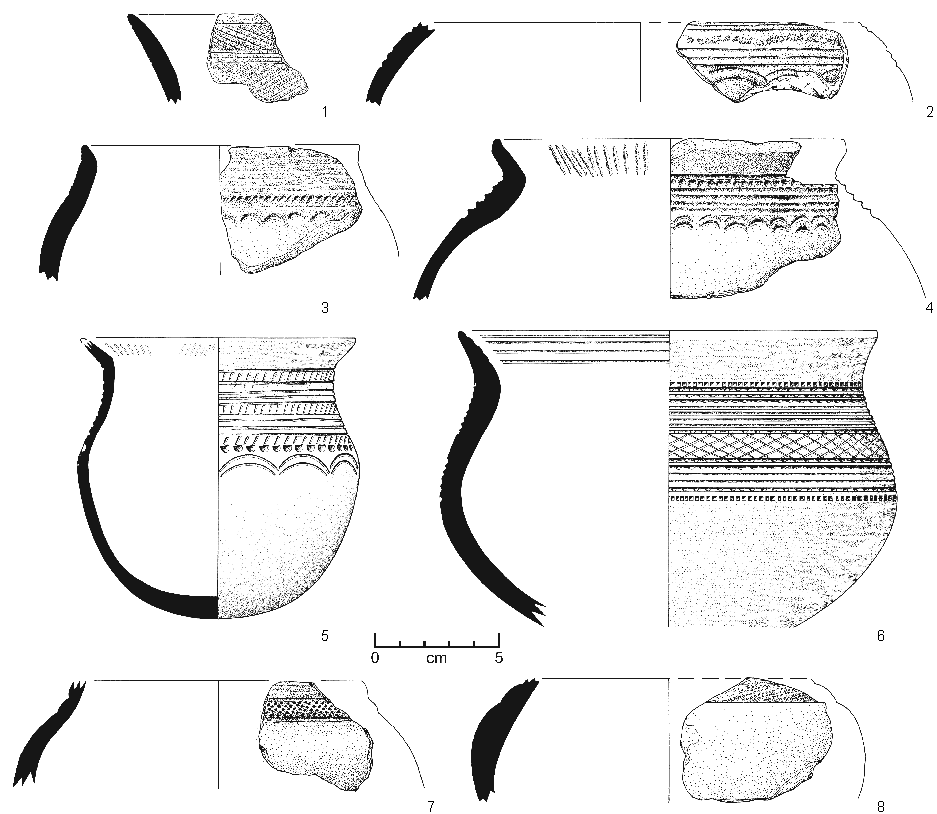
\includegraphics[width=.925\textwidth]{fig/NGB-Typen.pdf}
	\caption{\mbox{Ngbanja}-Gruppe: Typvertreter.\\1:~Taf.~58.14; 2:~Taf.~60.14; 3:~Taf.~6.10; 4:~Taf.~6.6; 5:~6.8; 6:~Taf.~6.7; 7:~Taf.~47.20; 8:~Taf.~6.9.}
	\label{fig:NGB_Typverteter}
\end{figure*}

\subsubsection{\mbox{Ngbanja}-Gruppe}\label{sec:NGB-Gr}

Eine deutliche Ähnlichkeiten zur Batalimo-Maluba-Keramik (siehe Kap.~\ref{sec:BTM-Gr}) aufweisende, sich von dieser jedoch auch deutlich unterscheidende Keramik findet sich vor allem entlang des mittleren und unteren \mbox{Ubangi}. Funde der, nach der Fundstelle \mbox{Ngbanja} (Fpl.~199) am mittleren \mbox{Ubangi} benannten Stilgruppe sind bislang fast ausschließlich aus Oberflächenabsammlungen bekannt. Die aus Grabungen bekannten Stücke machen zusammen 10\,\% aller der \mbox{Ngbanja}-Gruppe zugewiesenen GE aus.\footnote{1985 wurden bei den Grabungen in Maluba am Lua (Fpl.~230) zwei GE erfasst, deren Zuweisung zur \mbox{Ngbanja}-Gruppe jedoch fraglich ist. Bei den Grabungen in Pikunda am mittleren \mbox{Sangha} (Fpl.~255) wurden 1987 vier weitere GE ausgegraben. Eine sichere Einordnung dieser Stücke in die \mbox{Ngbanja}-Gruppe ist jedoch ebenfalls fraglich.} In den entsprechenden Inventaren bilden diese aber in jedem Fall isolierte Einzelfunde. Ein Befund, in dem die \mbox{Ngbanja}-Keramik dominiert, wurde bislang nicht erfasst. Neben der chronologischen Stellung lässt sich daher auch das formale Spektrum der Stilgruppe nur bedingt beschreiben. Folglich kann die \mbox{Ngbanja}-Gruppe beim gegenwärtigen Quellenstand lediglich als Provisorium angesehen werden.\footnote{Siehe auch \textcite[185\,f., 202]{Wotzka.1995} zur Zuweisung von nur spärlich in den im untersuchten Inventar belegten, aber charakteristischen keramischen Formen zu \enquote{Stilgruppen} mit provisorischem Charakter.\label{ftn:ProvisorischeStilGr}}

Insgesamt liegen 60~GE vor, die der \mbox{Ngbanja}-Gruppe zugewiesen wurden, wobei lediglich 20~GE als sicher der Stilgruppe zugehörig angesprochen wurden. Die zweifelsfrei der \mbox{Ngbanja}-Gruppe zugewiesenen Stücke stammen von lediglich sechs Fundstellen entlang des mittleren \mbox{Ubangi} sowie oberen \mbox{Sangha} (Abb.~\ref{fig:NGB_Verbreitung}): \mbox{Ngbanja} (Fpl.~199), Nzambi (Fpl.~205), Pikunda (Fpl.~255), Matoto (Fpl.~264), Ouesso (Fpl.~265) und Pandama (Fpl.~276). Bereits \textcite[140\,f. Fig.~13.4--5]{Eggert.1987c} war sich über die genaue Zuordnung der im Rahmen dieser Arbeit unter der Bezeichnung \mbox{Ngbanja} subsumierten Keramik nicht sicher. Einerseits sah er klare Ähnlichkeiten zur Keramik von Batalimo und Maluba, andererseits jedoch auch ebenso deutliche Unterschiede zu dieser.\footnote{Siehe Anm.~\ref{ftn:BTM-NGB-Unterschiede}.} Die fraglichen Formen konnten aufgrund der seit 1987 unveränderten Datenlage auch in der vorliegenden Auswertung nicht abschließend klassifiziert werden. Hier können, wie bereits auch von \textsc{Eggert} (ebd. 141) festgestellt, nur neue Grabungen eine Abhilfe schaffen.

\paragraph{Technologische Merkmale}\hspace{-.5em}|\hspace{.5em}%
Die Keramik der \mbox{Ngbanja}-Gruppe weist eine auffällige technologische Vielfalt auf. Das Material wird von Vertretern der \textit{Fabrics} 4a (23\,\%) und 4c (19\,\%) bestimmt, die zusammen knapp die Hälfte aller Funde abdecken. Ebenfalls häufig kommen die \textit{Fabrics} 5c (12\,\%) sowie 5b (8\,\%) vor. Wie auch bei der Keramik der Batalimo-Maluba-Gruppe (Kap.~\ref{sec:BTM-Gr}) dominieren die an mineralischen nichtplastischen Partikeln reichen und aus rotbrennenden Tonen gefertigten \textit{Fabrics} 4 und 5. Dies bedeutet, dass die GE viel bis sehr viel nichtplastisches Material (ca.~80\,\%) enthalten, das sich vor allem aus heterogenen Mischungen von Quarzsanden (>~80\,\%) zusammensetzt. In einigen Fällen ließen sich auch Laterit sowie Glimmer oder ausgebrannte Organik in den Scherben beobachten. Die Oberflächen der 20~GE, die sicher der \mbox{Ngbanja}-Gruppe zugewiesen wurden, schwankt zwischen rau und gut geglättet. An einigen Fundstellen, so an der namensgebenden Fundstelle \mbox{Ngbanja} (Fpl.~199), sind die Oberflächen eher gut geglättet, während sie in Nzambi (Fpl.~205) eher rau sind. Die mittlere Wandungsdicke der Scherben der \mbox{Ngbanja}-Gruppe liegt bei 7,3\,mm, bei einer Varianz von 2,9\,mm. Präferenzen bei der Auswahl der genutzten Tone bezüglich ihrer Brennfarbe ließen sich nicht erkennen. Während Scherben aus eindeutig rotbrennenden Tonen einen großen Anteil einnehmen (38\,\%) sind auch Stücke aus weißbrennenden Tonen in nicht unerheblichen Maße vertreten (23\,\%).


\paragraph{Formen}\hspace{-.5em}|\hspace{.5em}%
Insgesamt konnte lediglich bei acht von 26~GE, bei denen eine Ansprache der Gefäßform grundsätzlich möglich war, die Gefäßform auch sicher bestimmt werden. Das Formenspektrum wird von leicht bauchigen Gefäßen mit schwach ausgeprägter Schulterpartie bestimmt (Typ~C1; Abb.~\ref{fig:NGB_Typverteter}.2--3,5--8). Insgesamt sind 13~GE des Typs C1 bekannt, diese machen zusammengenommen mehr als 60\,\% aller mit einer Gefäßform angesprochenen GE aus. Bauchige Gefäße mit einem deutlich herausgearbeiteten Schulterbereich (Typ C2), die für die Batalimo-Maluba-Gruppe so charakteristisch sind, fanden sich im Material der \mbox{Ngbanja}-Gruppe lediglich ein Mal. Es konnten auch nur sehr wenige offene Gefäßformen beobachtet werden. Unter den 27~GE, bei denen eine Randform angesprochen werden konnte, entfällt mehr als die Hälfte auf einfache (B1) oder leicht konkav ausbiegende Ränder (B2). Die Ränder weisen in der Regel eine spitz zulaufende (M2; 27\,\%) oder gerillte Randlippe (M4; 20\,\%) auf. Lediglich bei einer, sicher der \mbox{Ngbanja}-Gruppe zuweisbaren GE konnte ein runder Boden (B1) beobachtet werden (Abb.~\ref{fig:NGB_Typverteter}.5). Bei zwei GE, die jedoch nicht zweifelsfrei der \mbox{Ngbanja}-Gruppe angehören müssen, wurden hingegen flache Standböden vom Typ B4 festgestellt. Auf dieser Basis kann keine Aussage getroffen werden, ob die \mbox{Ngbanja}-Keramik, wie die Batalimo-Maluba-Keramik, grundsätzlich als flachbodig bezeichnet werden kann.


\paragraph{Verzierungen}\hspace{-.5em}|\hspace{.5em}%
Das bestimmende Verzierungselement der \mbox{Ngbanja}-Gruppe sind horizontale Rillen (Tab.~\ref{tab:Verzierungselemente}: 02.1), die 45\,\% aller beobachteten Verzierungen ausmachen. Diese fanden sich bis auf die Gefäßunterteile und Böden an allen Gefäßpositionen in gleichem Maße (Anlage~4\subref{fig:NGB_Verz}). Auffällig sind das regelmäßige Auftreten innenseitig gerillter Ränder, ein Merkmal, das die \mbox{Ngbanja}-Keramik mit der Batalimo-Maluba-Keramik teilt. Anders als diese, weisen aber auch die Außenseiten der Ränder häufig Verzierungen auf. Diagonale Schachbrettmuster (Tab.~\ref{tab:Verzierungselemente}: 01.2) bilden mit 9\,\% aller Verzierungselemente die zweithäufigste Verzierung und sind regelhaft am Rand (Abb.~\ref{fig:NGB_Typverteter}.1) sowie den Schulterbereichen der Gefäße zu finden (Abb.~\ref{fig:NGB_Typverteter}.6). Kammeindrücke (Tab.~\ref{tab:Verzierungselemente}: 05.1; 7\,\%) sowie horizontale Reihen aus bogenförmigen Eindrücken (Tab.~\ref{tab:Verzierungselemente}: 04.19; 6\,\%) können ebenfalls beobachtet werden. Letztere lassen sich vornehmlich unterhalb der Rillenzier auf der Schulter- beziehungsweise Bauchpartie der Gefäße als untere Abschluss der Verzierungszone finden (Abb.~\ref{fig:NGB_Typverteter}.2, 4--5, Taf.~6.10). Horizontale Reihen aus Eindrücken (4.12) sind bei einigen GE zu beobachten (Abb.~\ref{fig:NGB_Typverteter}.6). Zwei GE zeichnen sich durch eine flache horizontale Leiste (Tab.~\ref{tab:Verzierungselemente}: 09.2) mit Kammeindrücken (Tab.~\ref{tab:Verzierungselemente}: 05.1) aus (siehe Abb.~\ref{fig:NGB_Typverteter}.7--8). Es handelte sich um die einzige Verzierung der entsprechenden GE.\footnote{Die auffällige Ähnlichkeit der beiden Stücke stellt einen vagen Bezug zwischen den beiden Fundstellen \mbox{Ngbanja} am mittleren \mbox{Ubangi} (Fpl.~199; Abb.~\ref{fig:NGB_Typverteter}.8) und Pikunda am mittleren \mbox{Sangha} (Fpl.~250; Abb.~\ref{fig:NGB_Typverteter}.7) her. Da keine eindeutige Vergesellschaftung dieser beiden Stücke mit anderen Formen des \mbox{Ngbanja}-Stils belegt ist, muss ihre Zuweisung jedoch fraglich bleiben. In \mbox{Ngbanja} selbst konnte aufgrund starker Fragmentierung der Surveyfunde mehr als die Hälfte aller GE keiner Stilgruppe zugewiesen werden. Unter den Stücken, die stilistisch angesprochen werden konnten, macht das Material der \mbox{Ngbanja}-Gruppe den größten Anteil aus.} An Gefäßunterteilen, Bodenansätzen und Standflächen konnte bei keiner der der \mbox{Ngbanja}-Gruppe zugewiesenen GE eine Verzierung beobachtete werden. 


\paragraph{Datierung}\hspace{-.5em}|\hspace{.5em}%
Das unter der Bezeichnung \mbox{Ngbanja} subsumierte keramische Fundgut stammt fast ausschließlich von Oberflächensurveys und Angaben zur Datierung der Stilgruppe können lediglich indirekt erfolgen. Einzig in der älteren Grube B1/B2 in PIK~87/1 (Kat.-Nr.~8) in Pikunda am \mbox{Sangha} fanden sich neben der für den Befund charakteristischen Pikunda-Munda-Keramik (Kap.~\ref{sec:PKM-Gr}) einige wenige, möglicherweise der \mbox{Ngbanja}-Gruppe zuweisbare Scherben (Tab.~\ref{tab:PIK87-1bis9_nichtPIK-MUN}). Diese können als Datierungsindiz gewertet werden, sind aber aufgrund mangelnder Sicherheit in der Bestimmung nur ein sehr schwacher Anhaltspunkt. Die drei GE sind mit Keramik der Pikunda-Munda-Gruppe sowie einer Scherbe der Lusako-Gruppe \parencite[Kap.~\ref{sec:LUS-Gr};][104--107]{Wotzka.1995} vergesellschaftet und werden durch eine Radiokohlenstoffdatierung zwischen das 4.~Jh. v.~Chr. und 3.--4.~Jh. n.~Chr. datiert (Tab.~\ref{tab:PIK87-1_Datierungen}: KI-2877).

\begin{figure*}[p]
	\centering
	\includegraphics[width=\textwidth]{fig/NGB_Verbreitung.pdf}
	\caption{\mbox{Ngbanja}-Gruppe: Verbreitung.}
	\label{fig:NGB_Verbreitung}
\end{figure*}

Da die Keramik der \mbox{Ngbanja}-Gruppe in keiner Grabung hinreichend nachgewiesen werden konnte, beruhen Angaben zur chronologischen Stellung der Keramik fast ausnahmslos auf losen, sich aus Vergleichen auf Merkmalsebene ergebenden Indizien. Mit Blick auf die formalen Charakteristika der \mbox{Ngbanja}-Keramik fallen deutliche Ähnlichkeiten zur Batalimo-Maluba-Gruppe auf (Kap.~\ref{sec:BTM-Gr}). \textcite[140\,f.]{Eggert.1987c} weist auf deutliche Unterschiede eines Gefäßes aus Ebeka (Taf.~5.7)\footnote{Das von \textsc{Eggert} (1987b: 140\,f., 142 Abb.~12.1; Taf.~5.7) aufgeführte Gefäß aus Ebeka wurde in der vorliegenden Analyse weder sicher der \mbox{Ngbanja}- noch der Batalimo-Maluba-Gruppe zugerechnet. Die Grundform des Gefäßes (siehe Abb.~\ref{Fig-BatMLB-Typvertreter}.6) sowie die die Verzierung bildenden Muster, vornehmlich das auffällige Zickzack-Band auf dem Gefäßbauch (siehe Abb.~\ref{Fig-BatMLB-Typvertreter}.5), weisen auf eine Nähe zur Batalimo-Maluba-Keramik hin. Ähnliche Gefäßformen sind aber auch aus der \mbox{Ngbanja}-Gruppe belegt (Abb.~\ref{fig:NGB_Typverteter}.4). Gerade die mangelnde Sorgfalt, mit der die Verzierungen auf dem Gefäß aus Ebeka aufgebracht sind, grenzt es jedoch vom Batalimo-Maluba-Stil ab, dessen Gefäße sich durch technisch äußerst sorgfältige und fein gearbeitete Verzierungen auszeichnen. Auch die Verzierung der Innenseite des Randes mit einem feinen diagonalen Schachbrett ließ sich bei keiner GE der Batalimo-Maluba-Gruppe beobachten. Das gleiche gilt für die breiten Rillen auf dem Gefäßhals. Entsprechende Parallelen finden sich jedoch in Formen der \mbox{Ngbanja}-Gruppe (Abb.~\ref{fig:NGB_Typverteter}.3). Diese Mischung aus Charakteristika verhinderte eine sichere Zuweisung des Gefäßes zu einer der beiden Stilgruppen.\label{ftn:BTM-NGB-Unterschiede}} sowie der Gefäße aus \mbox{Ngbanja} (Abb.~\ref{fig:NGB_Typverteter}.5--6) zur jüngeren Keramik entlang des mittleren \mbox{Ubangi} hin. Zur älteren Batalimo-Maluba-Keramik grenzen sich die angeführten Stücke vor allem durch den am Gefäß aus \mbox{Ngbanja} zu beobachtenden runden Boden ab (Abb.~\ref{fig:NGB_Typverteter}.5). \textsc{Eggert} (ebd. 141) hebt jedoch zugleich hervor, dass auch die flachen Böden der Batalimo-Maluba-Gruppe teilweise nur wenig abgesetzt sind und daher einen abgerundeten Eindruck vermitteln können. Mit der Batalimo-Maluba-Gruppe hat die \mbox{Ngbanja}-Keramik die Nutzung diagonaler Schachbrettmuster gemein (Tab.~\ref{tab:Verzierungselemente}: 01.2), die bei der \mbox{Ngbanja}-Gruppe jedoch deutlich grober ausgeführt sind. Die innen gerillten Ränder der \mbox{Ngbanja}-Keramik finden sich auch im Fundgut der Stilgruppen Batalimo-Maluba (Kap.~\ref{sec:BTM-Gr}) sowie Dongo (Kap.~\ref{sec:DON-Gr}). Gemeinsam mit der Dongo-Keramik hat die \mbox{Ngbanja}-Keramik rillenverzierte Gefäßhälse sowie girlandenartig umlaufende, bogenförmige Rillen (siehe Abb.~\ref{fig:DON_Typverteter}.8), grenzt sich von dieser aber auch durch die deutlich unterschiedliche Randgestaltung ab.

Zusammenfassend kann festgehalten werden, dass die \mbox{Ngbanja}-Gruppe eine ritzverzierte, eher grobe Keramik beschreibt, die stilistische Ähnlichkeiten zur ältesten Stilgruppe entlang des \mbox{Ubangi}-Gebietes, der Batalimo-Maluba-Gruppe, aufweist und unter Hinzuziehung einer Radiokohlenstoffdatierung aus Pikunda am Sangha (KI-2877) vorläufig in das 4.~Jh. v.~Chr. bis 3.--4.~Jh. n.~Chr. datiert werden kann. Dass die hauptsächlich mit Keramik der Pikunda-Munda-Gruppe (Kap.~\ref{sec:PKM-Gr}) assoziierte Radiokohlenstoffdatierung aus Pikunda für den vor allem am unteren Ubangi belegten \mbox{Ngbanja}-Stil als repräsentativ angesehen werden kann, gründet auf zwei nahezu identischen Scherben aus Ngbanja und Pikunda (Abb.~\ref{fig:NGB_Typverteter}.7--8). Vergleichbare Stücke fanden sich an keinem anderen Fundplatz im gesamten Arbeitsgebiet. Die unter der Bezeichnung \mbox{Ngbanja} subsumierte Keramik kann -- unter Vorbehalt -- als Phänomen der frühen Eisenzeit im Arbeitsgebiet und zumindest als teilweise zeitgleich zu den Stilgruppen Batalimo-Maluba (Kap.~\ref{sec:BTM-Gr}) wie Pikunda-Munda (Kap.~\ref{sec:PKM-Gr}) angesehen werden.

\paragraph{Verbreitung}\hspace{-.5em}|\hspace{.5em}%
Keramik, die der \mbox{Ngbanja}-Gruppe zugewiesen wurde, fand sich an 13 Fundplätzen, vornehmlich im Zentrum des Arbeitsgebietes (Abb.~\ref{fig:NGB_Verbreitung}). Sicher der \mbox{Ngbanja}-Gruppe zugewiesene Stücke fanden sich an lediglich sechs dieser 13 Plätze. Entlang des mittleren \mbox{Ubangi} sind dies der eponyme Fundplatz \mbox{Ngbanja} (Fpl.~199) und Nzambi (Fpl.~205), während Nbganja-Keramik weiter westlich, am mittleren bis oberen \mbox{Sangha} aus Pikunda (Fpl.~255), Matoto (Fpl.~264), Ouesso (Fpl.~265) sowie Pandama (Fpl.~276) bekannt ist. Mehr als ein Vertreter der \mbox{Ngbanja}-Gruppe fand sich lediglich in \mbox{Ngbanja} und Nzambi am mittleren \mbox{Ubangi} sowie Ouesso und Ikelemba (Fpl.~260) am mittleren \mbox{Sangha}; letztere Funde sind jedoch lediglich unter Vorbehalt der Stilgruppe zuzuweisen. Das Verbreitungsgebiet der \mbox{Ngbanja}-Gruppe ist insofern außergewöhnlich, da sich dieser Stilgruppe zugeordnete Keramik jeweils an den mittleren Flussläufen des \mbox{Ubangi} und \mbox{Sangha} findet, nicht jedoch im Mündungsgebiet der beiden Flüsse (Abb.~\ref{fig:NGB_Verbreitung}). Die Gebiete sind folglich nicht über die Flüsse miteinander verbunden. Dieses Verbreitungsbild gibt Grund zur Vorsicht und zukünftige Feldforschung muss zeigen, ob sich die Zuweisung der hier subsumierten Formen zu einer Stilgrupppe aufrecht erhalten lässt.

Akzeptiert man die \mbox{Ngbanja}-Gruppe und ihr Verbreitungsgebiet, so fällt auf, dass sie sich etwas weiter südlich als die Keramik der Batalimo-Maluba-Gruppe (Abb.~\ref{fig:BTM-Verbreitung}) findet, jener Stilgruppe, der die bislang ältesten, hinreichend belegten Spuren keramischer Erzeugnisse im \mbox{Ubangi}- und Lua-Gebiet zuzuordnen sind. Die chronologische Ansprache der \mbox{Ngbanja}-Keramik deutet auf eine hypothetische Gleichzeitigkeit dieser beiden Stilgruppen sowie der Pikunda-Munda-Gruppe des \mbox{Sangha}- und Likwala-aux-Herbes-Gebiets hin. Mit Bezug auf die Pikunda-Munda-Gruppe (Abb.~\ref{fig:PIKMUN_Verbreitung}) fällt auf, dass sich die Funde des \mbox{Ngbanja}-Stils entlang des \mbox{Sangha} eher stromauf finden. Zieht man die Kartierung der Regenwaldrefugien nach \textcite[7 Abb.~4]{Maley.2001} hinzu, so lässt sich erkennen, dass die Batalimo-Maluba-Gruppe im Norden außerhalb des postulierten Refugiums zu finden ist, während die Pikunda-Munda-Keramik im westlichen Teil des Refugiums verortet werden müsste. Die Fundpunkte der \mbox{Ngbanja}-Gruppe zeichnen hingegen den nordöstlichen Rand des Regenwald-Refugiums im Kongobecken nach. 